\typeout{IJCAI-11 Instructions for Authors}
\documentclass{article}
\usepackage{SortingNetworks}
\usepackage{times}
\usepackage{latexsym} 
\usepackage{pgfplots} % LaTeX
\usepackage{capt-of}
\usepackage[dutch]{babel}
\usepackage{amsthm}
\usepackage{amssymb}
\usetikzlibrary{arrows,automata}
\newtheorem{lemma}{Lemma}
\newtheorem{definitie}{Definitie}
\usepackage{subcaption}
\usepackage{listings}
\usepackage{color}
\usepackage{wrapfig}
\usepackage{tabu}

\definecolor{dkgreen}{rgb}{0,0.6,0}
\definecolor{gray}{rgb}{0.5,0.5,0.5}
\definecolor{mauve}{rgb}{0.58,0,0.82}
\lstset{frame=tb,
  language=Java,
  aboveskip=3mm,
  belowskip=3mm,
  showstringspaces=false,
  columns=flexible,
  basicstyle={\small\ttfamily},
  numbers=none,
  numberstyle=\tiny\color{gray},
  keywordstyle=\color{blue},
  commentstyle=\color{dkgreen},
  stringstyle=\color{mauve},
  breaklines=true,
  breakatwhitespace=true,
  tabsize=1
}
\renewcommand{\lstlistingname}{Code}

\title{Sorteernetwerken van Optimale Grootte}%\thanks{Dankwoord}}
\author{Mathias Dekempeneer, Vincent Derkinderen \\
Bachelor Informatica\\
Katholieke Universiteit Leuven \\
{voornaam.achternaam}@student.kuleuven.be}

\begin{document}

\maketitle

\begin{abstract}
Korte samenvatting van wat we doen en wat de conclusie is.\\
Verder werken op paper van Codish et al. Sorteer optimal size sorting network.\\
Tijdsverbetering van x?
Bla\\
Bla\\
Bla\\
Bla\\
Bla\\
Bla\\
Bla\\
Bla\\
Bla\\
Bla\\
Bla\\
\end{abstract}

\section{Introductie}

Situering + bijdrage.\\
Sorting Network (high level), Optimal Size (high level), contributies andere papers rond deze twee, enkele getallen rond grootte orde van het probleem, wat er al geprobeerd is (SAT, generate \& prune,...), hoe wij het probleem zullen aanpakken (hoe wij prunen (high level)), gebruikte hardware...\\
Bla\\
Bla\\
Bla\\
Bla\\
Bla\\
Bla\\
Bla\\
Bla\\
Bla\\
Bla\\
Bla\\
Bla\\
Bla\\
Bla\\
Bla\\
Bla\\

\section{Probleemstelling}
Een \textit{comparator netwerk} $C^n_k$ bestaat uit $n$ kanalen en $k$ \textit{comparatoren}.
Een comparator $\left(i, j\right)$ verbindt twee verschillende kanalen $i$ en $j$ waarbij $0 < i < j \leq n$.
We nemen $x_l^m$ als waarde op kanaal $m$ net voor comparator $l$, deze waarde is een element uit een totaal geordende set. 
De $l^{de}$ comparator  vergelijkt de huidige waarden van beide kanalen en plaatst de kleinste waarde op kanaal $i$ en de grootste waarde op kanaal $j$ zodat $x_{l+1}^i = \min(x_l^i,x_l^j)$ en $x_{l+1}^j = \max(x_l^i,x_l^j)$.
De uitvoer van een comparator netwerk verwijst naar de partieel geordende vector $\vec{x} = \{x^1_{k+1} \dots x^n_{k+1} \} $.
De invoer wordt voorgesteld door $\vec{x} = \{x^1_{0} \dots x^n_{0} \} $. 

Een \textit{sorteernetwerk} is een comparator netwerk met als eigenschap dat de uitvoer gesorteerd is ongeacht de invoer.
Een sorteernetwerk $C^n_k$ van optimale grootte houdt in dat er geen ander sorteernetwerk $C^n_l$ bestaat waarbij $l < k$. %TODO grootte = aantal comparatoren
Figuur \ref{Werking} is een voorbeeld van zo een netwerk waarop ook de werking gedemonstreerd wordt.
Deze figuur toont ook twee parallelle comparatoren $(1,2)$ en $(3,4)$, comparatoren die geen kanaal gemeenschappelijk hebben en van volgorde omgewisseld kunnen worden.
\begin{figure}[h!]
\centering
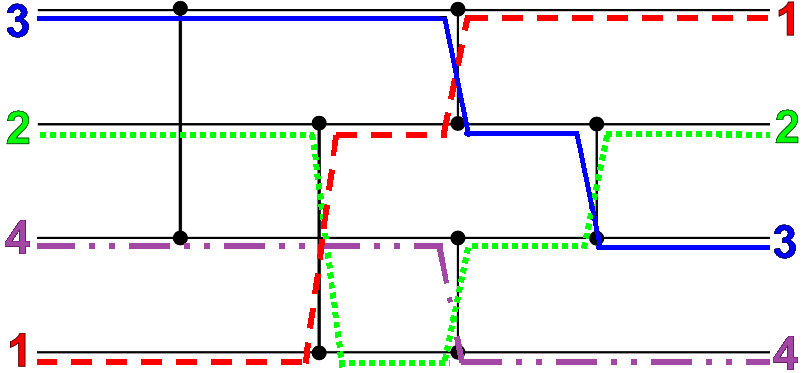
\includegraphics[scale=0.275]{NetworkTransparent.png} 
\caption{Sorteernetwerk 4 kanalen, 5 comparatoren}
\label{Werking}
\end{figure}
%TODO Hard enter?
Om te onderzoeken of een comparator netwerk een sorteernetwerk is, kunnen we gebruik maken van het \textit{nul - \'e\'en principe}. 
Dit principe, zoals beschreven volgens Knuth \cite{Knuth3}, stelt dat wanneer een comparator netwerk met $n$ kanalen alle $2^n$ mogelijke sequenties van $n$ $0$- en $1$-en sorteert, het een sorteernetwerk is.
De optimale grootte van een sorteernetwerk met $n$ kanalen is reeds bewezen tot en met $n \leq 10$ (Tabel \ref{tabel1} \cite{sortingNetworksSize2014}).
\begin{table}[h!]
\centering
\begin{tabular}{r|c|c|c|c|c|c|c}
n & 6 & 7 & 8 & 9 & 10 & 11 & 12\\ 
\hline 
bovengrens & 12 & 16 & 19 & 25 & 29 & 35 & 39\\ 
\hline 
ondergrens & 12 & 16 & 19 & 25& 29 & 33 & 37\\
\end{tabular} 
\caption{Minimaal aantal comparatoren bij $6 \leq n \leq 12$ kanalen.}
\label{tabel1}
\end{table}
%TODO Hard enter?
Voor $n > 10$ zijn er bovengrenzen gekend door zowel concrete voorbeelden als de systematische constructie van Batcher \cite{sortingNetworksApplications}. 
De ondergrenzen werden gevonden via bewijzen en lemma \ref{lemma1} \cite{Voorhis1972}.
\begin{lemma}
$S(n+1) \geq S(n) + \lceil \log_2(n) \rceil, \forall n \geq 1$
\label{lemma1}
\end{lemma}

\newcommand*\rfrac[2]{{}^{#1}\!/_{#2}}
\section{Voorgestelde oplossing}
Om te bewijzen dat een sorteernetwerk $C^n_k$ een sorteernetwerk is van optimale grootte, moeten we bewijzen dat er geen sorteernetwerk $C^n_{k-1}$ bestaat.
Aangezien $n$ kanalen zorgen voor $\frac{n \left(n-1\right)}{2}$ verschillende comparatoren, kunnen er $\left(\rfrac{n \left(n-1\right)}{2}\right) ^k$ verschillende netwerken gevormd worden met  $k$ comparatoren.
Voor $9$ kanalen en $24$ comparatoren betekent dit $2.245 \times 10^{37}$ verschillende netwerken, dit maakt het overlopen van alle netwerken niet aantrekkelijk.
%TODO Aaneenpraten
Door gebruik te maken van symmetrie\"en willen we snoeien in het aanmaken van deze netwerken.

We gebruiken de \textit{genereer- en snoei-methode} zoals beschreven door Codish \textit{et al.} (sectie 3, \cite{sortingNetworksSize2014}).
Deze methode heeft een cyclisch verloop waarbij men bij elke cyclus de set $R^n_k$ uitbreidt naar $N^n_{k+1}$ om vervolgens te snoeien en de set $R^n_{k+1}$ te bekomen (Figuur \ref{GenereerSnoei}).
\begin{figure}[!h]
\centering
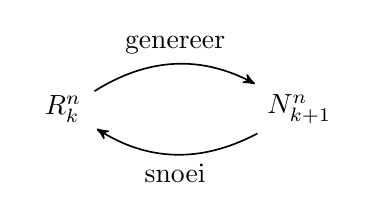
\begin{tikzpicture}[->,>=stealth',shorten >=1pt,auto,node distance=3cm,semithick]
  \tikzstyle{every state}=[fill=white,draw=none,text=black]

  \node[state] (A)                    {$R^n_k$};
  \node[state] (B) [right of=A] {$N^n_{k+1}$};

  \path (A) edge [bend left] node {genereer} (B)
  		  (B) edge [bend left] node {snoei} (A);
\end{tikzpicture}
\caption{Genereer en snoei principe}
\label{GenereerSnoei}
\end{figure}
Specifiek zullen we vertrekken van een netwerk zonder comparatoren om te eindigen bij $R^n_k$ bestaande uit \'e\'en sorteernetwerk van optimale grootte.
Bij de genereer-stap zullen we aan elk netwerk van $R^n_k$ alle mogelijke comparatoren toevoegen zodat $|N^n_{k+1}| = |R^n_{k}| \times \frac{n\left(n-1\right)}{2}$.
%TODO aanelkaarpraten zin misschien aanpassen)
Bij de snoei-stap zullen we dan netwerken verwijderen volgens het subsumes principe beschreven in definitie \ref{definitie1}.
\begin{definitie}[Subsumes] %TODO VRAGEN SUBSUMES => TOM NEDERLANDS/ENGELS
We zeggen ``Comparator netwerk $C^n_{k,a}$ subsumes comparator netwerk $C^n_{k,b}$'' wanneer een permuntatie $\pi$ bestaat zodat ${\pi\left(outputs\left(C_{a}\right)\right) \subseteq outputs\left(C_{b}\right)}$. Dit wordt genoteerd als $ C_{a} \preceq C_{b}$ om aan te duiden dat er een permutatie $\pi$ bestaat zodat $C_{a}\leq_\pi C_{b}$. %TODO Vincent weent om dit te kunnen herzien
\label{definitie1}
\end{definitie}
\begin{lemma}
Wanneer voor comparator netwerk $C^n_{k,a}, C^n_{k,b}$ geldt dat $ C_{a} \preceq C_{b}$ en er bestaat een sorteernetwerk $C_b;C$\footnote{$C_b;C$ is een concatenatie van netwerk $C_b$ en $C$.} van grootte $m$ dan bestaat er ook een sorteernetwerk $C_a;C'$ van grootte $m$.
\label{lemma2}
\end{lemma}
Concreet kunnen we de definitie van subsumes en lemma \ref{lemma2} beschreven door Codish \textit{et al.} \cite{sortingNetworksSize2014} gebruiken om in te zien dat we netwerken die gesubsumed worden door andere netwerken kunnen verwijderen.
Wanneer een set van netwerken een sorteernetwerk bevat, zal het snoeien van deze set resulteren in het bekomen van het sorteernetwerk.
Dit kan gebruikt worden om de eindigheid van het algoritme aan te tonen.

Het overlopen van alle permutaties om na te gaan of er een permutatie $\pi$ bestaat zodat ${\pi\left(Outputs\left(C_{a}\right)\right) \subseteq Outputs\left(C_{b}\right)}$, en dus $C_a \preceq C_{b}$, is een kostelijke bewerking.
Om deze bewerkingen te vermijden en te versnellen, zullen we extra methoden moeten invoeren om snellere beslissingen te maken over het ``subsumen van een ander netwerk''. 

\subsection{Representatie van comparator netwerken}
Bij de representatie van comparator netwerken moeten we rekening houden met geheugengebruik en de mogelijkheid om effici\"ente bewerkingen te kunnen uitvoeren.
Concreet zullen we comparatoren voorstellen door een sequentie van bits, waarbij twee bits op \'e\'en staan. Bijvoorbeeld  $ \left[ 0 1 0 0 1 0 \right]$ stelt de comparator $\left(2,5\right)$ voor bij een netwerk van $6$ kanalen.
Om de hoeveelheid overbodige bits te beperken, zullen we bij de \texttt{Java} implementatie gebruik maken van shorts\footnote{In \texttt{Java} bestaat een short uit $16$ bits.}.
Buiten de comparatoren worden ook de outputs van het netwerk bijgehouden, opgedeeld per aantal $1$'en. %TODO OUTPUTS - UITVOEREN?
In de \texttt{Java} implementatie kiezen we er voor om een comparator netwerk voor te stellen door een tweedimensionale array van shorts, short[][], en laten we de rij van $n$ $1$'en weg.
Een voorbeeld van zo een representatie staat in tabel \ref{tabel2}.
\begin{table}[!h]
\centering
\begin{tabular}{r|ccc}
Comparators & $\left[0011\right]$ & $\left[1010\right]$ & \\ 
\hline 
Outputs \'e\'en 1& $\left[0001\right]$ & $\left[0100\right]$ & $\left[0010\right]$ \\ 
\hline 
Outputs twee 1'en &$\left[0011\right]$ & $\left[0101\right]$ & $\left[0110\right]$\\ 
\hline 
Outputs drie 1'en & $\left[0111\right]$ & $\left[1011\right]$ &  \\ 
\end{tabular}
\caption{Representatie $C^4_2$: $(1,2)(2,4)$}
\label{tabel2}
\end{table}

\subsection{Genereren}
\begin{wrapfigure}{r}{0.12\textwidth}
	\vspace{-15pt}
	\begin{subfigure}[b]{0.10\textwidth}
	\centering
    		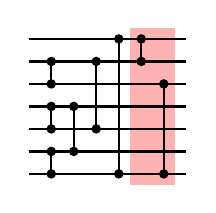
\begin{tikzpicture}
			\def\x{3.5}
			\fill [red!30] (4.5/\x,0.5/\x) -- (6.5/\x,0.5/\x) -- (6.5/\x,7.5/\x) -- (4.5/\x,7.5/\x) -- cycle;
			\foreach \a in {1/\x, 2/\x, 3/\x, 4/\x, 5/\x, 6/\x, 7/\x}
			\draw[thick] (0,\a) -- ++(7/\x,0);
			\foreach \b in {{1/\x,1/\x},{1/\x,2/\x},{1/\x,3/\x},{1/\x,4/\x},{1/\x,5/\x},{1/\x,6/\x},{2/\x,2/\x},{2/\x,4/\x},{3/\x,3/\x},{3/\x,6/\x},{4/\x,1/\x},{4/\x,7/\x},{5/\x,6/\x},{5/\x,7/\x},{6/\x,1/\x},{6/\x,5/\x}}
			\filldraw (\b) circle (1.5 pt);
			\draw[thick] (1/\x,1/\x) -- (1/\x,2/\x);
			\draw[thick] (1/\x,3/\x) -- (1/\x,4/\x);
			\draw[thick] (1/\x,5/\x) -- (1/\x,6/\x);
			\draw[thick] (2/\x,2/\x) -- (2/\x,4/\x);
			\draw[thick] (3/\x,3/\x) -- (3/\x,6/\x);
			\draw[thick] (4/\x,1/\x) -- (4/\x,7/\x);
			\draw[thick] (5/\x,6/\x) -- (5/\x,7/\x);
			\draw[thick] (6/\x,1/\x) -- (6/\x,5/\x);
		\end{tikzpicture}
		\caption{Netwerk 1}
		\label{fig1}
    \end{subfigure}
    
    \begin{subfigure}[b]{0.10\textwidth}
    \centering
		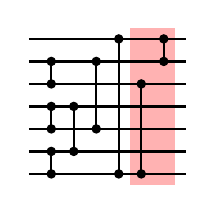
\begin{tikzpicture}
			\def\x{3.5}
			\fill [red!30] (4.5/\x,0.5/\x) -- (6.5/\x,0.5/\x) -- (6.5/\x,7.5/\x) -- (4.5/\x,7.5/\x) -- cycle;
			\foreach \a in {1/\x, 2/\x, 3/\x, 4/\x, 5/\x, 6/\x, 7/\x}
			\draw[thick] (0,\a) -- ++(7/\x,0);
			\foreach \b in {{1/\x,1/\x},{1/\x,2/\x},{1/\x,3/\x},{1/\x,4/\x},{1/\x,5/\x},{1/\x,6/\x},{2/\x,2/\x},{2/\x,4/\x},{3/\x,3/\x},{3/\x,6/\x},{4/\x,1/\x},{4/\x,7/\x},{6/\x,6/\x},{6/\x,7/\x},{5/\x,1/\x},{5/\x,5/\x}}
			\filldraw (\b) circle (1.5 pt);
			\draw[thick] (1/\x,1/\x) -- (1/\x,2/\x);
			\draw[thick] (1/\x,3/\x) -- (1/\x,4/\x);
			\draw[thick] (1/\x,5/\x) -- (1/\x,6/\x);
			\draw[thick] (2/\x,2/\x) -- (2/\x,4/\x);
			\draw[thick] (3/\x,3/\x) -- (3/\x,6/\x);
			\draw[thick] (4/\x,1/\x) -- (4/\x,7/\x);
			\draw[thick] (6/\x,6/\x) -- (6/\x,7/\x);
			\draw[thick] (5/\x,1/\x) -- (5/\x,5/\x);
		\end{tikzpicture}
		\caption{Netwerk 2}
		\label{fig2}
    \end{subfigure}
    \caption{}
    \vspace{-10pt}
\end{wrapfigure}
Bij de genereer-stap lopen we over de set $R^n_k$ en voegen we bij elk netwerk alle mogelijke comparatoren toe.
Aangezien een netwerk dat wordt uitgebreid met een overbodige comparator, \'e\'en waarbij de outputs ongewijzigd blijven, gesubsumed zal worden door een uitbreiding van dat netwerk met een niet overbodige comparator, kunnen we deze meteen verwijderen uit de set $N^n_{k+1}$. 
Alvorens deze beslissing te maken door alle outputs te overlopen, kunnen we ook eerst kijken of de comparator gelijk is aan de vorige in het netwerk.
%TODO zin bekijken: aaneenpraten
Wanneer 2 netwerken op de volgorde van hun parallelle comparatoren na gelijk zijn, zoals in figuur \ref{fig1} en \ref{fig2}, zullen deze elkaar subsumen en \'e\'en van de twee verwijderd worden.
Dit kan reeds bij de generatie-stap gemakkelijk opgevangen worden door bij het toevoegen van een nieuwe comparator x na te gaan of x een kanaal gemeenschappelijk heeft met de vorige comparator (Code \ref{code1}).
\begin{lstlisting}[caption={Test op parallelle comparatoren},label=code1]
x  & vorigeComp != 0
\end{lstlisting}
Wanneer dit niet het geval is en het dus parallelle comparatoren zijn, kunnen we bijvoorbeeld kiezen om het netwerk weg te gooien waarbij de nieuwe comparator kleiner is dan de vorige comparator.
%TODO Het vermelden van procesdata()

Tenslotte, na het toevoegen van de comparator, kunnen we de nieuwe outputs berekenen door de huidig bijgehouden outputs te gebruiken als invoer voor de nieuwe comparator.

\subsection{Snoeien}
Bij de snoei-stap lopen we over de set $N^n_{k+1}$ en verwijderen we alle netwerken die gesubsumed worden door een ander netwerk in de resterende set.
Om het aflopen van alle permutaties te vermijden, en sneller te beslissen of $C_a \preceq C_b$ met $C_a$ en $C_b$ twee comparator netwerken, voeren we enkele methoden in.
Zo gebruiken we onder meer lemma \ref{lemma3}, beschreven in de paper van Codish \textit{et al.}\cite{sortingNetworksSize2014}.
Bij $9$ kanalen wordt de methode $1.07666 \times 10^{13}$ keer uitgevoerd waarbij $1.05438 \times 10^{13}$ keer een beslissing genomen wordt. %TODO
\begin{lemma}
Wanneer het aantal outputs bij $C_a$ met $x$ $1$'en ($1 \leq x \leq n$) groter is dan bij $C_b$ weten we dat $C_a \npreceq C_b$ met $C_a$ en $C_b$ twee comparator netwerken.
\label{lemma3}
\end{lemma}
Voor lemma \ref{lemma4} van Codish (\cite{sortingNetworksSize2014}) introduceren we extra informatie over het comparator netwerk, namelijk $w\left(C_a, x, k\right)$ waarbij $x \in \{0,1\}$ en $0\leq k \leq n$.
Dit representeert de set van posities $i$ waarvoor er een output bestaat in $C_a$ met $k$ $1$'en waarvoor geldt dat op de $i^{de}$ positie van deze output een $x$ voorkomt. Om effici\"ent operaties te kunnen uitvoeren zullen we de posities voorstellen door middel van een bit representatie. Zo zal bijvoorbeeld $w\left(C_a, 1, 2\right) = 0110$ inhouden dat er bij de outputs met twee $1$'en minstens \'e\'en output bestaat met een $1$ op de $2^{de}$ positie, \'e\'en met een $1$ op de $3{de}$ positie en geen enkel met een $1$ op positie $1$ of $4$. Deze informatie voegen we bij elk netwerk toe in de vorm van een array van shorts, $w$. Elk kanaal $k$ van het netwerk $C_a$ vereist dan 4 opeenvolgende indices in $w$, zoals te zien in tabel \ref{tabel3}.
Deze informatie slaan we voor elk kanaal $k$ op vanaf index\footnote{In \texttt{Java} begint een array met index $0$.} $(k-1) \times 4$.
\begin{table}[!h]
\centering
\begin{tabu}{|[1.25pt]l|[1.25pt]c|[1.25pt]c|[1.25pt]c|[1.25pt]}
\tabucline[1.25pt]{-}
$w\left(C_a, 0, 1\right)$ & $|w\left(C_a, 0, 1\right)|$  & $w\left(C_a, 1, 1\right)$ & $|w\left(C_a, 1, 1\right)|$\\ 
\tabucline[1.25pt]{-}
\end{tabu} 
\caption{De inhoud van $w$ op indices $0-3$ voor kanaal 1.}
\label{tabel3} 
\end{table}
\begin{lemma}
Wanneer voor een comparator netwerk $C_a$ en $C_b$ met $n$ kanalen geldt dat $|w\left(C_a, x, k\right)| > |w\left(C_b, x, k\right)|$ voor $x \in \{0,1\}$ en $0 \leq k \leq n$ dan $C_a \npreceq C_b$.
\label{lemma4}
\end{lemma}
De methode van lemma \ref{lemma4} wordt bij $9$ kanalen ${2.22803 \times 10^{11}}$ keer uitgevoerd waarbij $2.05631 \times 10^{11}$ keer een beslissing genomen wordt.
%TODO te vaak van Codish et al. (centraliseer de verwijzing? of footnotes?)

Tenslotte komen we aan het nagaan van de permutaties.
Een na\"ieve methode zou zijn om alle $n!$ permutaties te overlopen.
In de plaats hiervan zullen we enkel permutaties afgaan die voldoen aan lemma \ref{lemma5}.
\begin{lemma}
${C_a \preceq C_b  \Rightarrow \pi\left(Outputs\left(C_{a}\right)\right) \subseteq Outputs\left(C_{b}\right)} \Rightarrow \pi\left(w\left(C_a, x, k\right)\right) \subseteq w\left(C_b, x, k\right)$, ${\forall x \in \{0,1\}, \forall k \in \{1..n\}}$.
\label{lemma5}
\end{lemma} 

\begin{lstlisting}[caption={Hallo},label=code2]
public boolean existsAValidPerm(short[][] network1, short[][] network2) {
	int allOnes = (1 << nbChannels) - 1;
	int[] posList = new int[nbChannels];
	
	for (int nbOnes = 1; nbOnes < nbChannels; nbOnes++) {
		int L2 = network2[nbChannels][(nbOnes << 2) - 2];
		int P2 = network2[nbChannels][(nbOnes - 1) << 2];
		
		int revLPos = allOnes ^ network1[nbChannels][(nbOnes << 2) - 2];
		int revPPos = allOnes ^ network1[nbChannels][(nbOnes - 1) << 2];
		
		if (L2 != allOnes || P2 != allOnes) {
			for (int i = 0; i < posList.length; i++) {
				int mask = 1 << i;
				if ((mask & L2) == 0) {
					posList[i] &= revLPos;
				}
				if ((mask & P2) == 0) {
					posList[i] &= revPPos;
				}
				if (posList[i] == 0) {
					return false;
				}
			}
		}
	}
	
	for (int i = 0; i < posList.length; i++) {
		int value = posList[i];
		if (Integer.bitCount(value) == 1) {
			for (int j = 0; j < posList.length; j++) {
				if (((value & posList[j]) != 0) && (i != j)) {
					posList[j] -= value;
					if (posList[j] == 0) {
						return false;
					}
				}
			}
		}
	}
	
	int checkAll = allOnes;
	for(int i = 0; i < posList.length; i++) {
		checkAll &= (~posList[i] & allOnes);
	}
	
	if(checkAll != 0) {
		return false;
	}
	
	return checkAllRelevantPermutations(network1, network2, posList, 0, new byte[nbChannels], 0);
}
\end{lstlisting}

~\\\\
Uitleg hoe we de prune doen.\\
Checken  van alle netwerken met alle netwerken voor de prune stap.
\begin{itemize}
\item Aantal 1en bij $C_a > C_b \Rightarrow C_a$ subsumes niet $C_b$ 
\item $|W(C_a, x, k)| > |W(C_b, x, k)| \Rightarrow C_a$ subsumes niet $C_b$
\item Uitleggen reductie van permutaties
\end{itemize}

\subsection{Parallellisatie}
Parallellisatie uitleggen\\
Uitleg hoe generate and prune verandert door elke thread zijn stuk te laten generate en prunen en vervolgens in een groter geheel te prunen en hoe dit groter geheel prunen werkt zonder locks.
%TODO ZIe pagina 4 in paper => definitie 2: Observe that ......

\section{Evaluatie}
Empirische evaluaties + grafiekjes\\
Tabel geven van hoeveel beslissingen er op welke plaats genomen worden.\\ \\
Vergelijken runtime voor 9 kanalen met Codish.\\
Schatting runtime voor 10 kanalen.\\\\

\begin{figure}[!h]
\centering
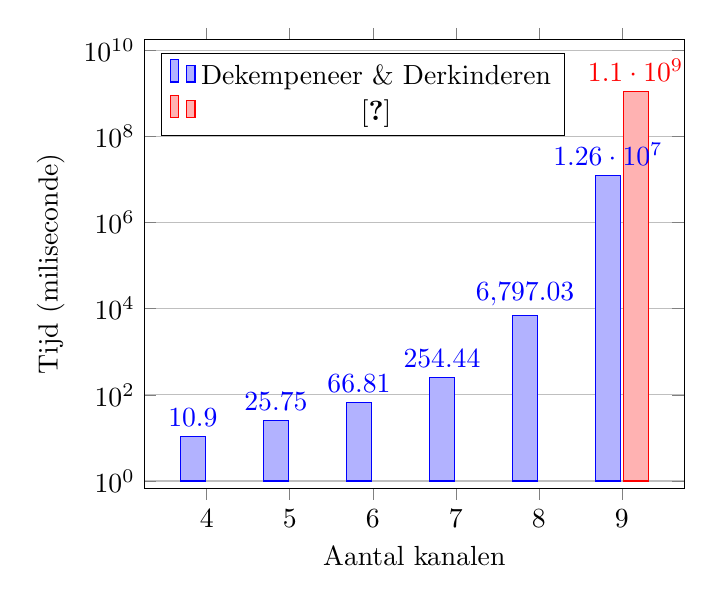
\begin{tikzpicture} 
	\begin{axis}[
		ylabel = Tijd (miliseconde),
		xlabel = Aantal kanalen,
		enlargelimits=0.15,
		ybar=1pt,
		ymode = log,
		log basis y = 10,
		bar width=9pt,
		nodes near coords,
		point meta=10^y,
		ymajorgrids = true, 
		legend pos = north west
]
%\addplot
%    coordinates {(4, 16.93) (5, 25.05) (6, 82.44) (7, 141.48) (8, 6680.31) (9, 15135358.01)};

\addplot
	coordinates {(4, 10.9026077) (5, 25.748741) (6, 66.820104) (7, 254.444729) (8, 6797.797437) (9, 12615521.409224)};	
	
\addplot
	coordinates {(9, 1101480000)};
	
\legend{Dekempeneer \& Derkinderen, \cite{sortingNetworksSize2014}};
\end{axis}
\end{tikzpicture}
\caption{Resultaten}
\end{figure}

\begin{figure}[!h]
\centering
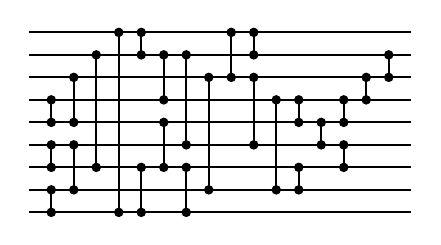
\begin{tikzpicture}
%\fill [gray!15] (1.5,1.5) -- (2.5,1.5) -- (2.5,2.5) -- (1.5,2.5) -- cycle;
%\foreach \a in {1,..,9}
\def\x{3.5}
\foreach \a in {1/\x, 2/\x, 3/\x, 4/\x, 5/\x, 6/\x, 7/\x, 8/\x, 9/\x}
  \draw[thick] (0,\a) -- ++(17/\x,0);
\foreach \b in {{1/\x,1/\x},{1/\x,2/\x},{1/\x,3/\x},{1/\x,4/\x},{1/\x,5/\x},{1/\x,6/\x},{2/\x,2/\x},{2/\x,4/\x},{2/\x,5/\x},{2/\x,7/\x},{3/\x,3/\x},{3/\x,8/\x},{4/\x,1/\x},{4/\x,9/\x},{5/\x,8/\x},{5/\x,9/\x},{5/\x,1/\x},{5/\x,3/\x},{6/\x,3/\x},{6/\x,5/\x},{7/\x,1/\x},{7/\x,3/\x},{6/\x,6/\x},{6/\x,8/\x},{7/\x,4/\x},{7/\x,8/\x},{8/\x,2/\x},{8/\x,7/\x},{9/\x,7/\x},{9/\x,9/\x},{10/\x,8/\x},{10/\x,9/\x},{10/\x,4/\x},{10/\x,7/\x},{11/\x,2/\x},{11/\x,6/\x}, {12/\x,2/\x},{12/\x,3/\x},{12/\x,5/\x},{12/\x,6/\x},{13/\x,4/\x},{13/\x,5/\x},{14/\x,3/\x},{14/\x,4/\x},{14/\x,5/\x},{14/\x,6/\x},{15/\x,6/\x},{15/\x,7/\x},{16/\x,7/\x},{16/\x,8/\x}}
  \filldraw (\b) circle (1.5 pt);
\draw[thick] (1/\x,1/\x) -- (1/\x,2/\x);
\draw[thick] (1/\x,3/\x) -- (1/\x,4/\x);
\draw[thick] (1/\x,5/\x) -- (1/\x,6/\x);
\draw[thick] (2/\x,2/\x) -- (2/\x,4/\x);
\draw[thick] (2/\x,5/\x) -- (2/\x,7/\x);
\draw[thick] (3/\x,3/\x) -- (3/\x,8/\x);
\draw[thick] (4/\x,1/\x) -- (4/\x,9/\x);
\draw[thick] (5/\x,8/\x) -- (5/\x,9/\x);
\draw[thick] (5/\x,1/\x) -- (5/\x,3/\x);
\draw[thick] (6/\x,3/\x) -- (6/\x,5/\x);
\draw[thick] (7/\x,1/\x) -- (7/\x,3/\x);
\draw[thick] (6/\x,6/\x) -- (6/\x,8/\x);
\draw[thick] (7/\x,4/\x) -- (7/\x,8/\x);
\draw[thick] (8/\x,2/\x) -- (8/\x,7/\x);
\draw[thick] (9/\x,7/\x) -- (9/\x,9/\x);
\draw[thick] (10/\x,8/\x) -- (10/\x,9/\x);
\draw[thick] (10/\x,4/\x) -- (10/\x,7/\x);
\draw[thick] (11/\x,2/\x) -- (11/\x,6/\x);
\draw[thick] (12/\x,2/\x) -- (12/\x,3/\x);
\draw[thick] (12/\x,5/\x) -- (12/\x,6/\x);
\draw[thick] (13/\x,4/\x) -- (13/\x,5/\x);
\draw[thick] (14/\x,3/\x) -- (14/\x,4/\x);
\draw[thick] (14/\x,5/\x) -- (14/\x,6/\x);
\draw[thick] (15/\x,6/\x) -- (15/\x,7/\x);
\draw[thick] (16/\x,7/\x) -- (16/\x,8/\x);
\end{tikzpicture}
\caption{Sorteernetwerk 9 kanalen, 25 comparatoren}
\end{figure}

\section{Conclusies}
Conclusie\cite{sortingNetworksSize2014}\\
Conclusie van wat er bereikt is en hoe er verder aan gewerkt kan worden.\cite{sortingNetworksTheEndGame}

\section*{Erkenning}
De rekeninfrastructuur en dienstverlening gebruikt in dit werk, werd voorzien door het VSC (Vlaams Supercomputer Centrum), gefinancierd door het FWO en de Vlaamse regering - departement EWI.\\
Professor Dr. Ir. Tom Schrijvers, Katholieke Universiteit Leuven.



\bibliographystyle{named}
\bibliography{SortingNetworks}

\end{document}

